\newpage
\subsection{Van Emde Boas trees}

\paragraph{Disposition}
\begin{itemize}
\item motivation and intuition.

\item small example (two insertions and a successor query).

\item $T(u) \leq T(\sqrt[\uparrow]{u}) + O(1)\ \in\ O(\lg \lg u)$.

\item illustrate how vEB operations follow this recurrence (examples for
  insert and successor).

\end{itemize}



\paragraph{Notes}

\begin{enumerate}

  \item hello.

  \item motivation for and intuition behind vEB trees.

  \item time and space complexity.\\

  \item vEB recurrence: $T(u) \leq T(\sqrt[\uparrow]{u}) + O(1)$.

  \item example for $U = 8$ (see \cref{fig:veb_example}).

  \item show $T(u) \leq T(\sqrt[\uparrow]{u}) + O(1) \in O(\lg \lg u)$.

  \item show how this recurrence describes vEB operations (insert and successor).

\end{enumerate}

\begin{figure}[H]
  \centering
  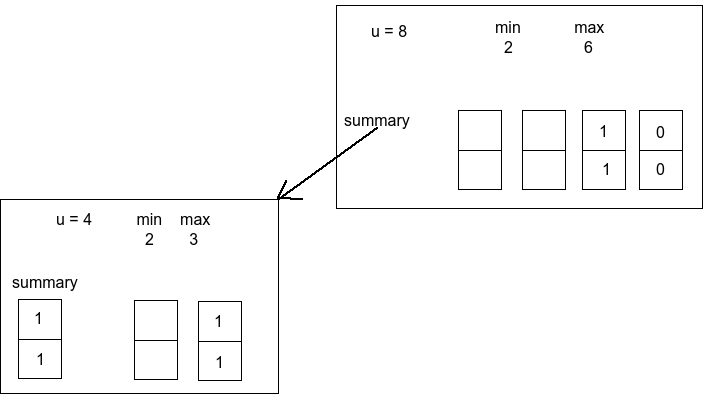
\includegraphics[width=0.7\textwidth]{figures/veb_example.png}
  \caption{Example -- vEB tree containing keys \{2, 5, 6\}.}
  \label{fig:veb_example}
\end{figure}
